\chapter{Methodology}
% information on the corpus and writing data
%define  features that I will use for classification how I decided on this and motivation behind these features.
%%%%%%%%%%%%%%%%%%%%%%%%%%%%%%%%%%%%%%%%
\section{Characteristics of Japanese}
%%%%%%%%%%%%%%%%%%%%%%%%%%%%%%%%%%%%%%%%

The agglutinative nature of Japanese coupled with the absence of explicit word delimiters, presents challenges for
accurate word segmentation. Furthermore, the use of three distinct writing systems
\footnote{Hiragana, Katakana, and Kanji} leads to considerable orthographic variation. for instance, learners at
lower proficiency levels frequently rely on the phonetic alphabets (hiragana and katakana), which can exacerbate
segmentation and tokenization errors. This phenomenon has been observed in previous studies
\citep{yang1998, nagata2009}, where systems demonstrated a lack of robustness against "spelling" errors or the
erroneous use of kanji.

Defining a "word" in Japanese also differs considerably from Indo-European languages. While a bound morpheme in
Enlgish might be treated as a indificual word. this is generally not the case in Japanese. For example,
segmentation can be difficult.
With 3
alphabets used there can orthographic variation is also fairly common. Learners at the lower proficentcy levels
mostly will write using the phonetic alphabets hiragana and katakana sometimes leading to errors in
segmentation/tokenization as was observed in \citep{yang1998, nagata2009}.

What is considered a word in Japanese may differ from other languages european languages. While a bound morpheme in
English might be treated
as an individual word, this is generally not the case in Japanese. For example, the word 話す\textit{hanasu}(to speak)
is considered a single word. However its potential form, 話せる \textit{hanaseru}(to be able to speak) is often analyzed as
two distinct morphemes: 話\textit{hana} and せる\textit{seru}. Initial abalyses using the chose tokenizer and parser
revealed inconsistencies in this regard. Similar inconsistencies were observed with compound verbs, such as
言い切る(\textit{iikiru}, "to completely say\footnote{\textit{to say without restraint}}"). While this was consistently
split into 言い(\textit{ii}"to say") and 切る(\textit{kiru} a suffix indicating completion), other instances were
segmented into
食べ (\textit{tabe}"to eat") 切る(\textit{kiru}"completely"). These inconsistencies pose significant hurdles for the
reliable extraction of specific grammatical forms for criterial features and can lead to unreliable counts for
complexity measures.
% maybe say something about taking this into consideration when writing rules for criterial features.

%%%%%%%%%%%%%%%%%%%%%%%%%%%%%%%%%%%%%%%%
\section{About the International Corpus of Japanese as a Second Language(I-JAS)}
%%%%%%%%%%%%%%%%%%%%%%%%%%%%%%%%%%%%%%%%

This study utilizes data from the International Corpus of Japanese as a Second Language (I-JAS), as
detailed in
\citet{Sakoda2020}, was
used.  The
I-JAS corpus is comprised of both spoken and written samples of Japanese.  It includes data from a diverse pool of 1,
000 adult learners
(aged
between 17 and 63 years old), all of whom are learning Japanese as a second language. 50 Native speaker samples are also
included in the corpus as a control group.

Participant's proficiency levels were assessed using the Japanese Computer Adaptive Test (J-Cat)
\citep{Imai2009}, with Further details about this assessment is provided in the
subsequent
section \ref{j-cat}. In addition to proficiency scores, the corpus includes various metadata for each participant,
such as
their
native language,
prior experience of visiting or living in Japan, and current geographical location (whether outside or within Japan).

%%%%%%% This part below contains information only on the essay writing samples I previously analyzed. I have also
%%%%%%% included additional writing samples added to the corpus which has brought the total particiapnt pool to 1000
%%%%%%% again.
Writing samples were extracted from the larger I-JAS corpus. Samples  were provided from 687 individuals, including the
control group
of 50 native speakers. A detailed breakdown of the of the participants in the writing sample subset, categorized by
their corresponding Japanese Language Proficiency Test (JLPT) levels, is presented in \ref{tab:participants-chart}.

%Name: count, dtype: int64
\begin{table}[h!]
\centering
\begin{tabular}{cc}
\hline \textbf{JLPT Proficiency Level} & \textbf{\# of Participants} \\ \hline
N5 & 176 \\
N4  & 318 \\
N3 & 297\\
N2 & 165 \\
N1 & 44 \\
Native Speakers & 50 \\
\hline
\end{tabular}
\caption{Distribution of participants across JLPT proficiency levels. J-cat scores have been mapped to their equivallent JLPT levels. }
\label{tab:participants-chart}
\end{table}

%%%%%%%%%%%%%%%%%%%%%%%%%%%%%%%%%%%%%%%%
\subsection{The Japanese Computerized Adaptive Test (J-CAT)}
\label{j-cat}
%%%%%%%%%%%%%%%%%%%%%%%%%%%%%%%%%%%%%%%%

%background and information on the J-CAT test compare to JLPT.

The Japanese Computerized Adaptive Test (J-CAT) \citep{Imai2009}, is a computer-administered assessment
designed to evaluate an
individual's proficiency in the Japanese language. While formerly freely accessible, the J-CAT is now overseen by
the  日本語教育支援協会(Japanese Language Education Support Association (JaLESA)). Japanese
universities frequently
employ the J-CAT as an efficient tool and flexible tool for placing foreign students into appropriate Japanese
language courses, primarily due to its on-demand administration compared to the JLPT which is only
administered bi-annually.

The adaptive nature of the J-CAT allows it to tailor question difficulty based on a student's performance across
four core areas: Vocabulary, Grammar, Listening, and Reading. Each participant receives a numberial score, which is
then mapped to one of seven distinct proficiency levels. These levels have been correlated with equivalent JLPT
scores, as detailed in \ref{tab:proficency-table}. For this study participants were categorized according to their
assigned JLPT level. Native speaker participants were assigned a default J-CAT score of 999.

\begin{figure}[h!]
    \centering
    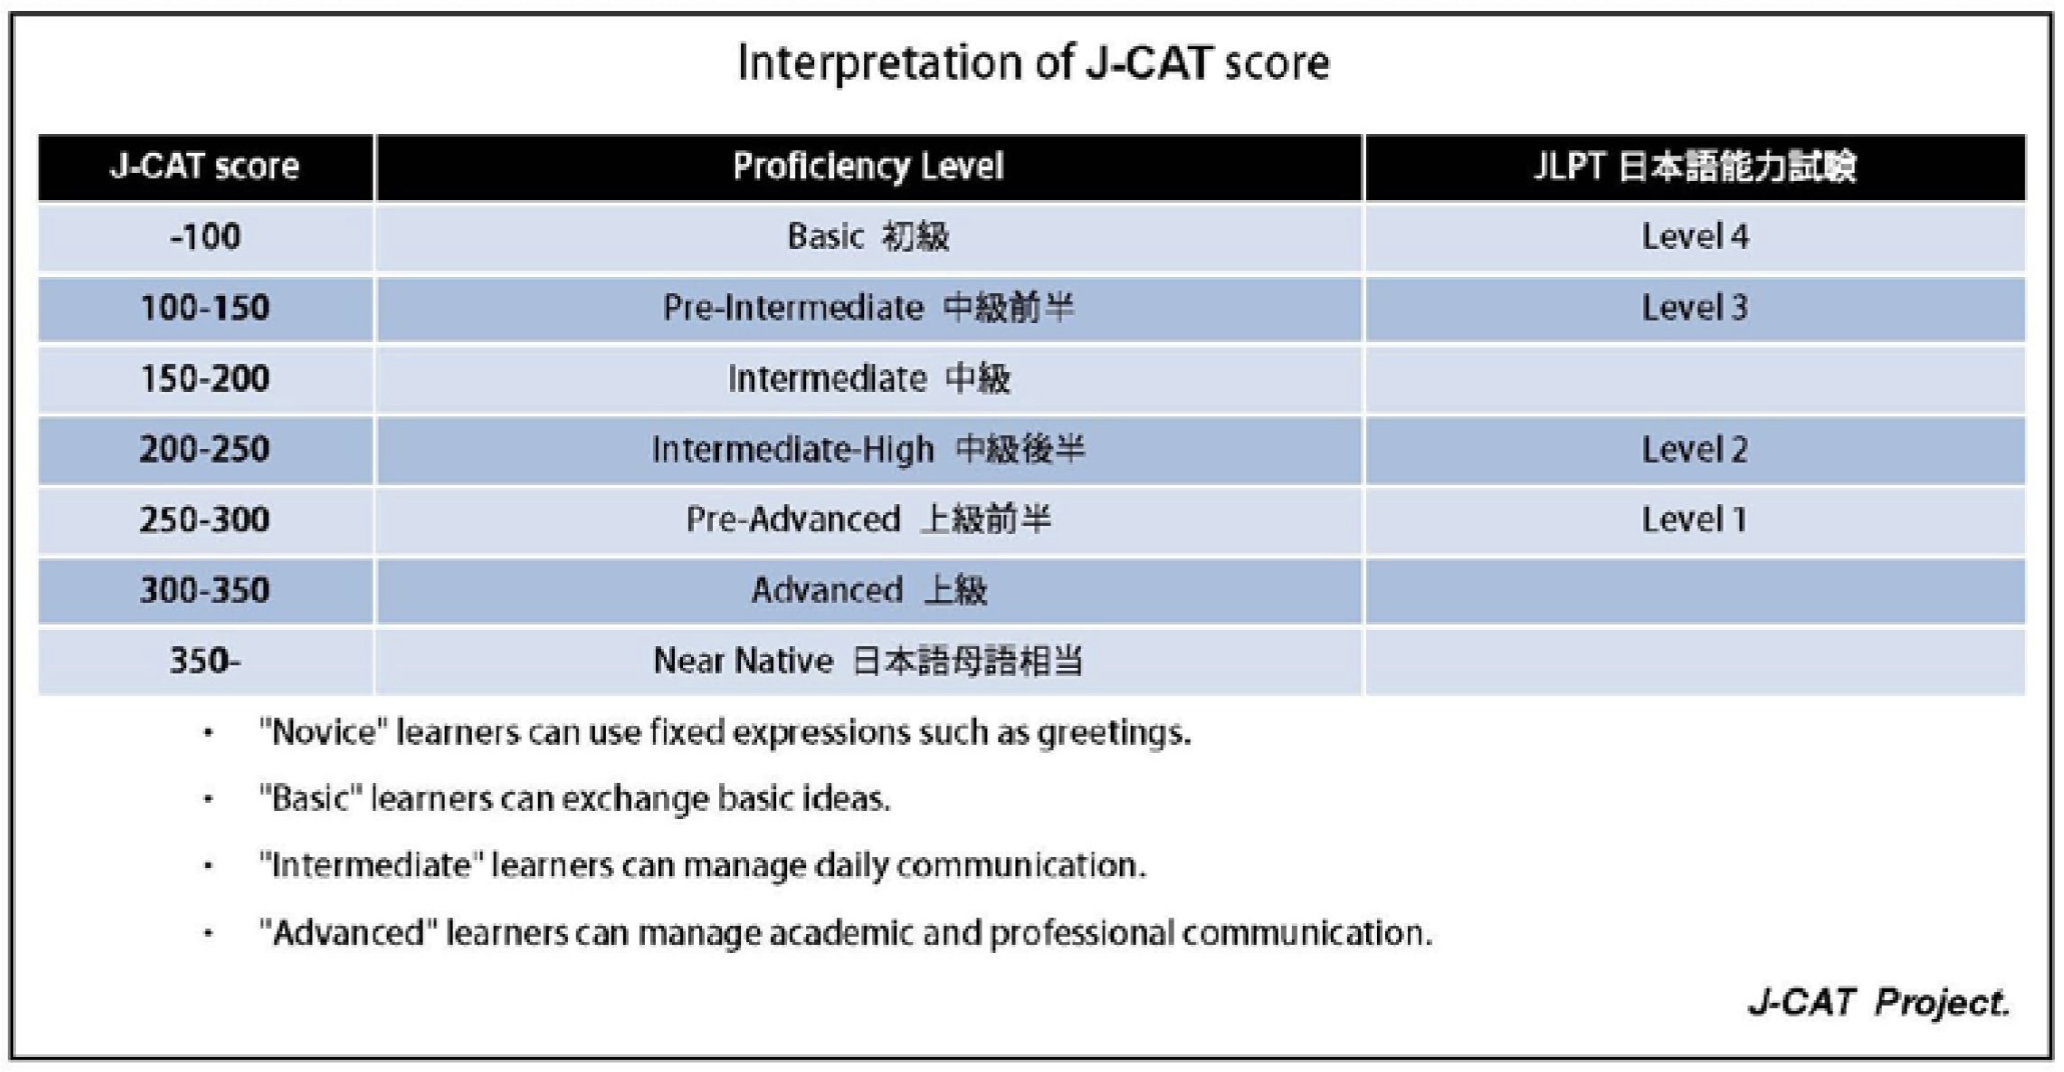
\includegraphics[scale=.3]{img/JCatScores.png}
    \caption{The assigned proficency levels from the J-Cat test as presented in the original paper in  2009. It is important to note that JLPT equivalencies do not align with the current JLPT framework, which was reformed in 2010. A revised score interpretation, connecting J-CAT scores to the updated JLPT levels, was released in 2011 and is provided in Table \ref{tab:proficency-table} }
    \label{fig:JCatLevels}
\end{figure}


\begin{table}[h!]
\centering
\begin{tabular}{lrl}
\hline \textbf{JLPT Proficiency Level} & \textbf{J-Cat Score}  \\ \hline
N5 & 0 - 149 \\
N4 & 150 - 199 \\
N3 & 200 - 249 \\
N2 & 250 - 299 \\
N1 & 300 - \\
Native & 999\\
\hline
\end{tabular}
\caption[Proficency Levels]{JLPT proficency level classification based on J-cat score ranges, adapted from
\cite{jcat_interpretation_guide}.}
\label{tab:proficency-table}
\end{table}

%%%%%%%%%%%%%%%%%%%%%%%%%%%%%%%%%%%%%%%%
\subsection{Writing Tasks}
%%%%%%%%%%%%%%%%%%%%%%%%%%%%%%%%%%%%%%%%

% add the additional SW 1 and 2 tasks where participants were expected to write a story based on a picture.
Each participant submitted up to six samples of writing for specific tasks, detailed below that were designed to
elicit a variety of linguistic responses across different discourse types and levels of formality:
\begin{itemize}
    \item (\textbf{Task e}), A short essay titled "Our Eating Habits," requiring a comparatie analysis of fast food
    and home-cooked
    meals within the context of the learner's home country.
    \item (\textbf{Task m1}), A formal letter addressed to a former teacher, requesting a letter of recommendation
    for a scholarship
    application.
    \item (\textbf{Task m2}), An email seeking an extension for a report submission deadline.
    \item An apology email (\textbf{m3}) declining an invitation to give a close friend a sight-seeing tour.
    \item (\textbf{Task SW1}), A story-telling task, where the learner was expected to narrate a story based on a
    series of pictures depicting a picnic theme. Sample images for this task are also shown in Figure \ref{fig:ST}
    in the appendix.
    \item (\textbf{Task SW2}), A story telling task where the learner was expected to narrate a story based on a
    series of pictures depicting a lost key. Sample images for this task can be seen in Figure \ref{fig:ST} in the
    appendix.
\end{itemize}

These tasks were standardized across all participants, regardless of their proficiency levels, encompassing a range
of communicative functions and formalities. Average text length can be see to vary widely across the task as shown
in figure \ref{fig:text-lengths}.
While the possibility of a "task
effect" as
observed in
\citet{Alexpoulou2017} is possible due to certain tasks requiring the use of certain forms, as the tasks are
consistent across proficiency levels,
this consistency allows for a direct observation of the linguistic forms learners use at different proficiency
levels across tasks. Consequently, all writing samples within the corpus were processed as-is, without any
correction of learner
errors.

\begin{figure}[h!]
    \centering
    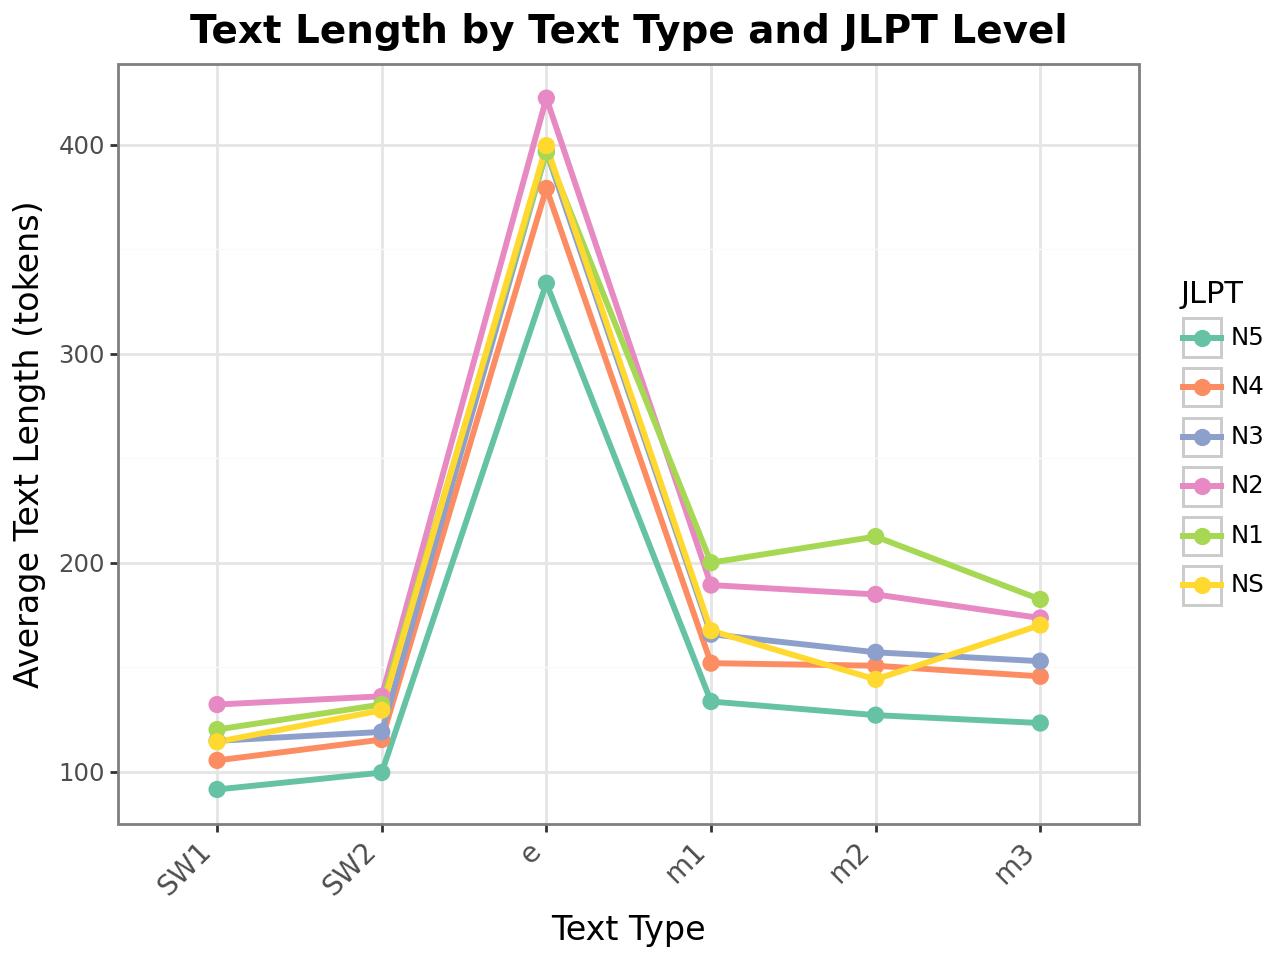
\includegraphics[scale=.5]{img/text_length_chart}
    \caption{The average text length across task and JLPT level. A detailed chart is
    included in the Appendix table \ref{tab:text_len}}
    \label{fig:text-lengths}
\end{figure}

%%%%%%%%%%%%%%%%%%%%%%%%%%%%%%%%%%%%%%%%
\subsection{Text Preprocessing}
%%%%%%%%%%%%%%%%%%%%%%%%%%%%%%%%%%%%%%%%

%Mention the preprocessing of the text. Talk about spacys' ginza pipeline used for parsing-tagging etc.
The raw text data from each writing sample underwent a comprehensive preprocessing pipeline. Given the specific
challenges of Japanese text processing, particularly for learner language where standard NLP tools may not be
robust, Spacy's Ginza package \cite{Ginza} (v 5.2) a Japanese language model for spaCy for Japanese was employed.
Ginza was selected for its comprehensive capabilities in handling Japanese text, including tokenization,
Part-of-Speech(POS) tagging, depedency parsing, lemmatization, morphological analysis, and its integration with
spaCy's rule based matcher.

For certain morphological lexical and measures, punctuation was removed from the text to prevent its influence on
token counts and other analyses. All characters in the writing were first converted to full-size characters \footnote{This is to prevent any errors due to unintentional half-size characters that may have been included in the writings when converting between different formating. For this the mojimoji package was used https://pypi.org/project/mojimoji/}, then
the texts were tokenized, tagged for parts-of-speech,
Lemmatizatized, dependency parsed.

The corpus for this study comprises over 4,840 uncorrected samples of writing from the participants, necessitating
the reliance on measures that can be automatically calculated.
 The algorithms for calculating various complexity measures and criterial features, discussed in subsequent
sections, were
were developed by the author based on the output of this preprocessing pipeline. The source code for these
algorithms in publicly available at: \href{https://github.com/meghorikawa/JFE}{https://github.com/meghorikawa/JFE} .

%%%%%%%%%%%%%%%%%%%%%%%%%%%%%%%%%%%%%%%%
\section{Complexity Measures}
%%%%%%%%%%%%%%%%%%%%%%%%%%%%%%%%%%%%%%%%
To capture the multifaced nature of language development, this study uses a multi-dimensional approach to complexity
measurement. Measures were chosen across multiple linguistic domains- including lexical, syntactic and morphological
complexity - at both gloabl and local levels. The following sections describe the specific measures chosen for each
domain. A comprehensive list of all complexity measures extracted in this study is located in the Appendix in
Table \ref{tab:complexity-measures}

%%%%%%%%%%%%%%%%%%%%%%%%%%%%%%%%%%%%%%%%
\subsection{Syntactic Complexity Measures}
%%%%%%%%%%%%%%%%%%%%%%%%%%%%%%%%%%%%%%%%
Syntactic complexity is assessed using a combination of global and local measures, which together provide a fuller
picture of learners' syntactic development. Global measures reflect complexity at the sentence or clause level,
and illustrate a learner's ability to build extended structures. Local measures focus on phrase-level elaboration
and the richness of internal units.

Due to the large size of the corpus, one of the main criteria for choosing these measures was the ease with which
they could be automatically calculated. For this reason, T-unit based measures, which require more complex and often
manual annotation, were not included.

\subsubsection{Global Measures}
Among the global measures, average sentence length and clauses per sentence were included. Sentence length is
calculated as the average number of tokens in each sentence, while clauses per sentence counts both finite and
non-finite clauses divided by the number of sentences. These measures indicate how much structural elaboration
learners achieve, as longer sentences/clauses indicate more units used.

In addition, the frequency of subordinate and coordinate clauses per sentence was used to examine learners' use of
clausal embedding.
Subordinate clauses represent hierarchical syntactic relationships (e.g. conditionals or complements),
while coordinate clauses reflect additive or sequential connections between clauses. These measures provide insight
into learners'
use of complex sentence structures. A similar method was employed in \citet{Vyatkina2012}, where the frequency of
subordinating and
coordinating conjunctions as a proxy for coordination and subordination
Following Vyatkina's approach, this study also uses the frequency of surface forms as a proxy for subordination and
coordination. To
allow for comparability across text of different lengths, these counts were normalized by total word count using the
following formula:
% this is the formula
\begin{center}
${\displaystyle \frac{\# \hspace{5pt} of \hspace{5pt}SC \hspace{5pt}or \hspace{5pt}CC}{total \hspace{5pt} \hspace{
5pt}word \hspace{5pt}count} }  * 100$
\end{center}
where SC and CC refer to subordinating and coordinating conjunctions, respectively.

However, automatically identifying subordinate and coordinate clauses in Japanese in challenging. The POS tag for
subordinating conjunctions (SCONJ) is often applied to particles that may function as coordinators or subordinators
depending on the context. Also, dependency labels that mark coordination are not always reliably assigned by parsers
due to ambiguity in structure \citep{UDJapanese}. Because of this, standard automatic annotation may not clearly
differentiate coordination from subordination in Japanese.

To work around this, a rule-based approach was used to approximate the frequencies of subordinate and coordinate
clauses. This method relies on detecting specific surface forms of conjunctions such as 「から」(kara) and 「ので」(node)
for subordination, or chains of te-forms for coordination. Although this may not capture non-standard constructions,
it is a practical way to estimate clause types in a large corpus.

\subsubsection{Local Measures}
On the local level, measures such as noun phrase length, verb phrase length, mean dependency distance (MDD), and mean
hierarchical
distance (MHD) were included. Noun phrase length is the average number of tokens per noun phrse, reflecting phrase
complexity, or more descriptiveness by adding adjectives to compliment nouns.  Similar to noun phrase length, verb
phrase length also analyzes the length of verb phrases and any adverbs, complementizers, used.  MDD and MHD,
indicate linear and hierarchical syntactic complexity and offer a more detailed view of sentence processing demands.

%%%%%%%%%%%%%%%%%%%%%%%%%%%%%%%%%%%%%%%%
\subsection{Lexical Complexity Measures}
%%%%%%%%%%%%%%%%%%%%%%%%%%%%%%%%%%%%%%%%
%Corrected Type Token Ratio
%Noun Density
%Verb Density (including auxilaries)
%Adjective Density
%Adverb Density
%MTLD
%Lexical Frequency Profile

Lexical complexity in this study is analyzed using both text internal measures and
text
external measures. Text internal measures are based solely on the vocabulary used within each text and measure the
diversity and density of the vocabulary in a text. In contrast, text-external measures assess sophistication by
comparing the vocabulary in a learner text to an external source such as a
frequency list or graded vocabulary resources.

\subsubsection{Text Internal Measures}
%internal
The internal measures selected for this study include the
Corrected-Type-Token-Ratio(CTTR),Measure of Textual Lexical Diversity (MTLD), and part of speech (POS) density
measures, including noun density, verb density(including auxiliaries), adjective density and adverb density.

CTTR is a refinement of the traditional type-token ratio that reduces sensitivity to text length. It is calculated
using the formula:
%%%%CTTR Formula
\begin{equation}
\begin{center}
    \centering CTTR = ${\displaystyle \frac{total \hspace{5pt} unique\hspace{5pt} words}{\sqrt{2*total words}} } $
\end{center}
\end{equation}
\vspace{5pt}

MTLD was used as a complementary measure of lexical diversity that is robust against text lengths. It calculates the
average length of word strings that maintain a minimum type-token ratio threshold, commonly .72 (this threshold was
also used in this study). A higher
MTLD
score indicates a more lexical diversity.

MTLD was implemented using a modified version of a
publicly
available
Python script \citep{MTLD_repo}. The script was adapted to support both surface-level and lemma-based calculation
modes and was integrated with the GiNZA tokenizer to handle Japanese texts. Punctuation was removed based on
spaCy's POS tags before
calculating the MTLD score. Because the measure is only sensitive to variation after a minimum number of tokens \citep{McCarthy2010},
texts with fewer than 50 tokens were excluded from MTLD calculation.

POS density measures were calculated by dividing the number of nouns, verbs(including auxiliaries), adjectives and
adverbs by the total
number of tokens in a given text. These measures provide insight into the functional distribution of lexical items and
descriptive elaboration used by learners.

%%%Formula of

\subsection{Text External Measures}
% External
%LFP - Using JLPT word lists BCCWJ
To assess lexical sophistication, the Lexical Frequency Profile (LFP) was implemented using two frequency based
resources:
\begin{itemize}
    \item The Balanced Corpus of Contemporary Written Japanese (BCCWJ) frequency list \citep{maekawa2014}, which
    provides frequency information for words appearing across a wide range of genres including books, magazine,
    blogs,
    internet
    forums, and textbooks.
    \item JLPT word lists, sourced from \citep{jisho.org}, classifies vocabulary into five levels from N5(
    basic) to N1 (advanced) based on the Japanese Language Proficiency Test (JLPT).
    \end{itemize}

In the LFP, each word in a learner text is categorized into a frequency band or JLPT level. The percentage of tokens
from each band is then calculated to assess the extent to which learners rely on high-frequency (common) versus
lower-frequency (uncommon) vocabulary  from
each of the bands.

To esure compatibility betwee the learner texts and the word lists, preprocessing was required. Word from the
frequency lists were tokenized using the same pipeline (GiNZA) as the learner texts to allow consistent matching.
 For example, some expressions such as
「もう一度」 (
\textit{mouichido}, "one more time") would appear as single entries in the vocabulary list but are tokenized
into separate
items(e.g. 「もう」and 「一度」) . By applying the same tokenizer to both the learner data and the frequency resources, this
mismatch was minimized.


%%%%%%%%%%%%%%%%%%%%%%%%%%%%%%%%%%%%%%%%
\subsection{Morphological Complexity}
%%%%%%%%%%%%%%%%%%%%%%%%%%%%%%%%%%%%%%%%
Morphological Complexity can be measured through two domains variation, which reflects the diversity of morphological
forms employed and
elaboration, which captures the internal complexity of those forms. Japanese, as an
agglutinative
language, with extensive verb inflection, auxiliary chaining, politeness marking, and compounding,
offers
numerous opportunities for both morphological variation and elaboration. To quantitatively evaluate these aspects, two
main
approaches were employed, the Morphological complexity index as proposed by
\citet{Brezina2019} and a Japanese adaptation of the Korean Readability Morphological Analyzer (JRMA) by
\citet{Hwang2024}.

The Japanese Readability Morphological Analyzer (JRMA), is based on the KRMA developed for Korean, another
agglulative language. The JRMA indentifies and counts morphological constructions that reflect
functional and grammatical elaboration in Japanese, including verb inflections, honorific and polite forms, and noun
formations.
Morphemes
are categorized into three distinct types for analysis: Content morphemes (e.g. nouns, verbs, adjectives ),
function
morphemes (
auxilaries, and particles), and all morphemes. For each of these categories two variation measures are
calculated: the
Measure of Textual Lexical Diversity (MTLD) and the Moving Average Type-Token Ratio (MATTR).

MATTR is calculated by sliding a fixed-size window (this study used a size of 50) across the text and computing the
type-token ratio (
TTR) with in each window. The final MATTR score represents the average of all windowed TTR values.

\begin{equation}
    \text{MATTR} = \frac{1}{N} \\sum_{i=1}^{N} \frac{\text{unique types}_i}{w}
\end{equation}

Here' N is the total number of windows, unique types, refers to the number of unique types in window \textit{i}, and
\textit{w} is
the
fixed window size.

An additional measure, auxiliary chain density was
developed to evaluate
morphological elaboration. This measure identifies auxilary-like elements that attach to main verbs, such as
auxiliary verbs (e.g.ます, ない), non-independent verbs(非自立動詞)(e.g. みる,おく), or conjunctive particles like 「て」and 「で. The
auxiliary chain density is and
computed as the
average the
number of these elements per main verb. This measure demonstrates how learners layer grammatical functions providing insight into their ability to produce structurally complex constructions.

As used in their original study, two forms of the Morphological Complexity Index (MCI) were implemented:
surface
MCI and
inflectional MCI. Surface MCI measures the diversity of the word forms at the token level, capturing variation
across all visible forms including conjugated verbs and inflected nouns. Inflectional MCI, on the other hand,
calculates the diversity of
the inflectional lemmas.

Calculation of the MCI is done by diving the text into consecutive segments of a fixed size,\textit{k}, (usually 5
or 10
tokens), and for each segment, a type token ratio (TTR) is calculated based on the number of unique surface forms in
that window. The final MCI score is the average of these TTRs across all segments.

\begin{equation}
    \text{MCI} = \frac{1}{N}\sum_{i=1}^{N} \frac{\text{Unique forms}_i}{k}
\end{equation}

Here, \textit{N} is the total number of segments, Unique Forms is the number of unique forms (surface or
inflectional) in segment \textit{i}, and \textit{k} is the fixed segment size.
%%%%%%%%%%%%%%%%%%%%%%%%%%%%%%%%%%%%%%%%
\section{Criterial Features}
%%%%%%%%%%%%%%%%%%%%%%%%%%%%%%%%%%%%%%%%

Describe the rule based feature matcher I made for extracting certain grammar patterns to disconcern their use
across proficiency levels. Mention how many grammar points at each level I was able to include. Use of the lower
levels doesn't disconcern much so focus should be on the intermediate and upper levels.  Forms that are mainly form
based(and therefore easier to pattern match) should be given priority over. Give some examples of rules derrived
%154 grammar points from JLPT have been annotated make a list for appendix

% add an example of the rules for matching
mention that I chose forms which spanned multiple levels. I.e. しか at N4 used with Nouns and しか〜ないat N3 used
with verbs to see if their use at the different levels actually follows this.

don't forget about implementing normalization.

Official documents with grammar from the different levels of JLPT do not exist however many 'unoffical lists' of
grammar, vocabulary, Kanji are available - including Jisho.org, personally compared againast published material from
ARUKU

A comprehensive list of all 154 grammar forms extract from the text is included in table \ref{
tab:Criterial-Features} in the appendix.


%%%%%%%%%%%%%%%%%%%%%%%%%%%%%%%%%%%%%%%%
\section{EBMS}
%%%%%%%%%%%%%%%%%%%%%%%%%%%%%%%%%%%%%%%%

 Overview was already done in Background section. Mention more details about training etc.


